\SourceLeaf{269}%
\noindent Endlich wird nach (C):
\[
QSR = 90^{0} - g(PQ) \,.\, RQS,
\]
demnach vermöge 7):
\[
QRS = 90^{0} - \frac{g(r)^2}{f(r)} \,.\, PQ
\]
und daher
\[
\tag*{(D)} \begin{aligned}PSR &= PSQ + QSR\\ &= 90^{0} + \frac{1 - g(r)^2}{f(r)} \,.\, PQ.\end{aligned}
\]

14. In dem Viereck $PQRS$ (Fig. 11) verlängere man $QR$ um das unendlich kleine
Stück $RR'$, errichte auf $QR'$ in $R'$ das Loth $R'S'$, das die Verlängerung von
$PS$ in $S'$ treffen möge, und trage auf $R'S'$ die Strecke $R'T = RS$ ab.

\begin{center}\begin{minipage}{\linewidth}\centering
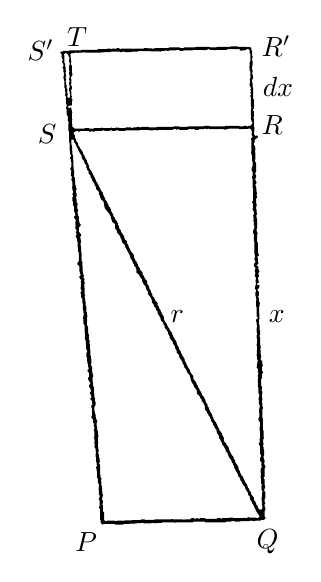
\begin{tikzpicture}[x=0.00731225cm,y=-0.00731225cm]
\fill[even odd rule] (410,56) -- (408,56) -- (407,57) -- (405,56) -- (390,56) -- (389,55) -- (377,55) -- (376,56) -- (353,56) -- (352,57) -- (341,57) -- (340,56) -- (316,56) -- (315,57) -- (296,57) -- (295,58) -- (289,58) -- (288,57) -- (270,57) -- (269,58) -- (245,58) -- (244,59) -- (227,58) -- (226,59) -- (209,59) -- (208,60) -- (206,59) -- (187,59) -- (185,60) -- (182,58) -- (180,58) -- (179,59) -- (171,59) -- (170,60) -- (168,59) -- (163,59) -- (162,60) -- (146,60) -- (145,61) -- (118,61) -- (117,62) -- (97,62) -- (96,63) -- (86,63) -- (85,64) -- (82,64) -- (81,65) -- (81,66) -- (83,68) -- (83,74) -- (85,78) -- (84,82) -- (86,86) -- (86,90) -- (85,91) -- (85,93) -- (86,94) -- (86,99) -- (87,100) -- (87,107) -- (86,108) -- (86,110) -- (87,111) -- (87,114) -- (88,115) -- (88,127) -- (89,128) -- (89,134) -- (90,135) -- (89,140) -- (91,143) -- (91,145) -- (90,146) -- (91,148) -- (91,155) -- (92,156) -- (92,160) -- (91,161) -- (91,163) -- (92,164) -- (92,173) -- (94,177) -- (94,185) -- (96,187) -- (95,189) -- (95,202) -- (96,203) -- (96,215) -- (97,216) -- (96,218) -- (96,221) -- (97,222) -- (97,236) -- (98,237) -- (98,242) -- (99,243) -- (99,247) -- (98,248) -- (98,250) -- (99,251) -- (99,255) -- (100,256) -- (100,264) -- (98,268) -- (100,271) -- (100,273) -- (99,274) -- (99,279) -- (101,282) -- (101,284) -- (100,285) -- (100,287) -- (102,291) -- (102,299) -- (101,301) -- (102,302) -- (102,305) -- (103,306) -- (103,310) -- (102,311) -- (102,313) -- (103,314) -- (103,316) -- (102,317) -- (102,324) -- (103,325) -- (103,331) -- (105,334) -- (105,342) -- (106,343) -- (106,346) -- (107,347) -- (107,349) -- (105,351) -- (105,353) -- (108,357) -- (108,359) -- (107,360) -- (107,365) -- (108,366) -- (107,368) -- (107,372) -- (109,374) -- (109,376) -- (108,377) -- (108,379) -- (109,380) -- (109,382) -- (108,383) -- (108,387) -- (110,389) -- (110,393) -- (111,394) -- (111,404) -- (112,405) -- (112,412) -- (113,413) -- (113,428) -- (110,433) -- (114,437) -- (114,446) -- (115,447) -- (115,450) -- (116,451) -- (116,453) -- (114,455) -- (114,457) -- (117,461) -- (117,463) -- (116,464) -- (117,466) -- (116,477) -- (118,479) -- (118,480) -- (116,482) -- (116,485) -- (117,486) -- (117,491) -- (119,494) -- (119,501) -- (120,502) -- (120,513) -- (121,514) -- (121,518) -- (122,519) -- (120,528) -- (121,529) -- (121,537) -- (123,540) -- (123,552) -- (124,553) -- (124,559) -- (123,561) -- (124,562) -- (124,565) -- (125,566) -- (126,581) -- (128,586) -- (126,588) -- (126,594) -- (127,595) -- (128,606) -- (129,607) -- (129,612) -- (130,613) -- (130,616) -- (128,618) -- (128,619) -- (131,623) -- (131,629) -- (129,631) -- (129,633) -- (131,637) -- (133,639) -- (133,641) -- (131,644) -- (131,647) -- (133,649) -- (133,651) -- (134,652) -- (134,655) -- (132,657) -- (132,658) -- (134,660) -- (134,662) -- (135,663) -- (135,665) -- (133,667) -- (133,668) -- (136,671) -- (136,675) -- (137,676) -- (137,677) -- (135,679) -- (135,683) -- (136,684) -- (136,697) -- (135,698) -- (135,700) -- (138,704) -- (138,709) -- (139,710) -- (139,715) -- (140,716) -- (140,720) -- (139,721) -- (139,723) -- (140,724) -- (140,733) -- (139,735) -- (140,736) -- (140,739) -- (141,740) -- (140,742) -- (140,746) -- (141,747) -- (140,751) -- (142,754) -- (142,759) -- (143,760) -- (143,762) -- (142,763) -- (142,768) -- (143,769) -- (143,777) -- (144,778) -- (144,782) -- (145,783) -- (145,784) -- (143,786) -- (143,788) -- (144,789) -- (144,793) -- (145,794) -- (145,805) -- (146,806) -- (146,813) -- (148,816) -- (148,823) -- (147,824) -- (148,826) -- (148,834) -- (149,835) -- (149,839) -- (148,840) -- (148,843) -- (149,844) -- (149,854) -- (148,856) -- (150,860) -- (150,877) -- (151,878) -- (151,883) -- (154,886) -- (156,885) -- (175,885) -- (176,886) -- (190,886) -- (191,885) -- (215,884) -- (216,883) -- (218,883) -- (219,884) -- (221,883) -- (225,883) -- (226,884) -- (238,884) -- (239,883) -- (243,883) -- (245,884) -- (247,883) -- (249,884) -- (250,883) -- (257,883) -- (258,882) -- (279,882) -- (280,883) -- (282,882) -- (311,882) -- (312,881) -- (332,881) -- (333,882) -- (368,882) -- (369,881) -- (377,881) -- (378,880) -- (384,880) -- (385,881) -- (393,881) -- (394,880) -- (410,880) -- (411,879) -- (419,880) -- (420,879) -- (429,879) -- (430,878) -- (434,878) -- (437,876) -- (437,873) -- (436,872) -- (436,862) -- (437,861) -- (437,856) -- (436,855) -- (436,850) -- (437,849) -- (436,847) -- (436,841) -- (437,840) -- (437,830) -- (435,827) -- (437,819) -- (436,818) -- (436,808) -- (434,806) -- (434,805) -- (436,803) -- (436,788) -- (437,787) -- (437,784) -- (435,781) -- (436,775) -- (435,774) -- (435,771) -- (434,770) -- (434,767) -- (435,766) -- (435,756) -- (434,755) -- (434,751) -- (433,750) -- (433,748) -- (434,747) -- (433,739) -- (435,735) -- (434,734) -- (434,723) -- (433,722) -- (433,702) -- (432,701) -- (432,685) -- (433,684) -- (433,682) -- (432,681) -- (432,675) -- (431,674) -- (431,671) -- (432,670) -- (432,666) -- (431,665) -- (432,655) -- (430,653) -- (431,651) -- (431,646) -- (430,645) -- (430,633) -- (431,632) -- (431,625) -- (433,622) -- (433,620) -- (431,618) -- (431,613) -- (433,609) -- (432,608) -- (432,603) -- (429,599) -- (429,597) -- (430,596) -- (430,592) -- (429,591) -- (429,583) -- (428,582) -- (429,580) -- (429,575) -- (428,574) -- (428,561) -- (427,560) -- (427,557) -- (428,556) -- (428,549) -- (427,548) -- (427,539) -- (426,538) -- (426,529) -- (427,528) -- (426,508) -- (427,507) -- (427,503) -- (428,501) -- (426,499) -- (426,493) -- (425,492) -- (425,489) -- (426,488) -- (426,482) -- (423,478) -- (426,475) -- (427,471) -- (426,470) -- (424,470) -- (422,468) -- (426,465) -- (424,457) -- (426,455) -- (425,449) -- (427,447) -- (425,442) -- (425,438) -- (422,436) -- (422,435) -- (425,433) -- (425,431) -- (424,430) -- (424,423) -- (423,421) -- (426,418) -- (426,417) -- (424,414) -- (424,396) -- (423,395) -- (423,382) -- (424,380) -- (422,376) -- (422,372) -- (423,371) -- (423,355) -- (422,354) -- (422,351) -- (421,350) -- (423,346) -- (422,344) -- (422,339) -- (421,338) -- (421,334) -- (422,333) -- (422,329) -- (421,328) -- (421,320) -- (423,317) -- (422,315) -- (422,312) -- (423,310) -- (422,309) -- (421,298) -- (420,297) -- (420,295) -- (422,292) -- (420,288) -- (420,284) -- (421,283) -- (421,279) -- (420,278) -- (420,274) -- (421,273) -- (421,258) -- (419,254) -- (419,252) -- (420,251) -- (420,240) -- (419,239) -- (420,231) -- (417,225) -- (417,223) -- (419,221) -- (418,218) -- (424,213) -- (424,210) -- (421,210) -- (420,211) -- (418,209) -- (418,207) -- (417,206) -- (417,204) -- (418,203) -- (418,195) -- (417,194) -- (417,192) -- (418,190) -- (417,189) -- (417,180) -- (416,179) -- (417,177) -- (417,168) -- (416,167) -- (416,164) -- (417,163) -- (417,160) -- (418,158) -- (417,157) -- (417,147) -- (416,146) -- (416,127) -- (415,126) -- (415,119) -- (414,118) -- (414,113) -- (416,110) -- (415,104) -- (414,103) -- (414,101) -- (415,100) -- (415,97) -- (414,96) -- (414,89) -- (415,88) -- (415,81) -- (414,80) -- (414,76) -- (415,75) -- (415,72) -- (414,71) -- (414,63) -- (413,62) -- (413,58) -- cycle
(101,217) -- (103,217) -- (105,219) -- (105,222) -- (107,224) -- (110,231) -- (112,233) -- (112,235) -- (115,241) -- (118,245) -- (118,248) -- (120,252) -- (122,254) -- (123,258) -- (126,262) -- (126,266) -- (127,267) -- (127,269) -- (130,272) -- (130,276) -- (133,279) -- (133,281) -- (136,286) -- (136,288) -- (140,293) -- (140,295) -- (143,300) -- (143,303) -- (148,308) -- (148,312) -- (150,315) -- (150,317) -- (152,321) -- (156,325) -- (158,336) -- (166,346) -- (169,352) -- (169,355) -- (170,356) -- (171,360) -- (176,364) -- (176,371) -- (179,375) -- (179,378) -- (185,385) -- (185,388) -- (187,390) -- (188,395) -- (193,400) -- (194,404) -- (202,419) -- (203,424) -- (205,426) -- (207,430) -- (207,432) -- (209,434) -- (209,436) -- (212,439) -- (212,441) -- (213,442) -- (213,448) -- (218,452) -- (219,455) -- (223,460) -- (223,463) -- (226,469) -- (229,472) -- (230,477) -- (233,481) -- (233,485) -- (237,490) -- (240,496) -- (240,500) -- (243,503) -- (244,507) -- (246,509) -- (248,514) -- (250,516) -- (250,519) -- (255,527) -- (255,530) -- (260,536) -- (260,538) -- (262,540) -- (262,544) -- (266,548) -- (268,552) -- (268,554) -- (271,559) -- (271,562) -- (276,568) -- (277,572) -- (280,576) -- (281,581) -- (283,583) -- (283,587) -- (287,591) -- (288,596) -- (293,603) -- (293,605) -- (296,610) -- (296,612) -- (300,617) -- (301,621) -- (306,627) -- (308,636) -- (310,640) -- (312,642) -- (313,646) -- (318,653) -- (318,658) -- (323,663) -- (324,666) -- (326,668) -- (327,672) -- (329,674) -- (332,680) -- (332,686) -- (335,689) -- (336,692) -- (338,694) -- (338,696) -- (341,699) -- (341,701) -- (343,703) -- (343,706) -- (346,710) -- (346,712) -- (349,716) -- (349,718) -- (352,721) -- (353,727) -- (356,731) -- (357,736) -- (359,738) -- (360,742) -- (362,744) -- (362,747) -- (365,750) -- (368,756) -- (368,758) -- (371,761) -- (374,769) -- (378,774) -- (379,778) -- (381,780) -- (381,782) -- (383,784) -- (383,787) -- (390,800) -- (390,802) -- (393,805) -- (394,809) -- (397,813) -- (397,815) -- (402,821) -- (402,823) -- (407,831) -- (407,834) -- (410,837) -- (411,843) -- (414,847) -- (414,849) -- (416,851) -- (422,864) -- (427,871) -- (427,872) -- (424,875) -- (422,875) -- (421,874) -- (409,874) -- (408,873) -- (407,873) -- (405,875) -- (401,875) -- (400,874) -- (398,875) -- (382,875) -- (381,874) -- (374,874) -- (373,875) -- (362,875) -- (361,876) -- (359,875) -- (354,875) -- (353,876) -- (333,876) -- (332,875) -- (324,875) -- (323,876) -- (317,875) -- (316,876) -- (314,876) -- (313,875) -- (309,875) -- (306,877) -- (297,877) -- (296,878) -- (294,877) -- (277,877) -- (275,876) -- (274,877) -- (245,877) -- (244,878) -- (228,878) -- (227,877) -- (222,877) -- (221,878) -- (191,879) -- (190,880) -- (188,879) -- (180,879) -- (179,880) -- (176,880) -- (175,879) -- (162,879) -- (161,880) -- (159,880) -- (157,878) -- (157,865) -- (155,863) -- (155,853) -- (154,852) -- (155,845) -- (153,843) -- (155,834) -- (154,833) -- (153,819) -- (152,818) -- (152,811) -- (151,810) -- (152,808) -- (152,805) -- (150,803) -- (151,801) -- (150,799) -- (150,782) -- (148,780) -- (150,776) -- (149,775) -- (149,770) -- (148,769) -- (148,764) -- (147,763) -- (147,759) -- (148,757) -- (147,756) -- (147,752) -- (146,751) -- (146,745) -- (147,744) -- (146,742) -- (146,734) -- (147,733) -- (147,730) -- (146,729) -- (146,723) -- (145,722) -- (145,716) -- (144,715) -- (144,709) -- (145,708) -- (145,705) -- (143,703) -- (143,700) -- (142,699) -- (142,694) -- (141,693) -- (141,690) -- (140,689) -- (140,682) -- (142,678) -- (142,673) -- (141,672) -- (141,666) -- (140,665) -- (140,659) -- (139,658) -- (139,647) -- (138,646) -- (138,643) -- (137,642) -- (138,640) -- (137,638) -- (137,630) -- (138,629) -- (138,626) -- (137,625) -- (137,622) -- (136,621) -- (136,612) -- (134,609) -- (134,607) -- (135,606) -- (135,599) -- (134,598) -- (134,593) -- (133,592) -- (133,582) -- (132,581) -- (132,572) -- (131,571) -- (132,567) -- (130,564) -- (131,562) -- (130,560) -- (131,557) -- (129,553) -- (129,543) -- (127,539) -- (127,532) -- (128,531) -- (127,529) -- (127,526) -- (128,525) -- (128,522) -- (127,521) -- (127,517) -- (126,516) -- (126,507) -- (125,506) -- (125,499) -- (124,498) -- (124,493) -- (123,492) -- (123,490) -- (124,489) -- (124,487) -- (123,486) -- (123,475) -- (122,474) -- (123,472) -- (122,470) -- (123,468) -- (123,464) -- (122,463) -- (123,460) -- (121,456) -- (122,453) -- (120,450) -- (119,429) -- (118,428) -- (118,423) -- (117,422) -- (118,420) -- (118,414) -- (117,413) -- (117,403) -- (116,402) -- (116,396) -- (117,395) -- (117,393) -- (116,392) -- (116,388) -- (115,387) -- (115,386) -- (117,384) -- (117,382) -- (113,377) -- (113,370) -- (116,367) -- (116,364) -- (114,362) -- (114,359) -- (113,358) -- (113,351) -- (112,350) -- (112,347) -- (111,346) -- (111,342) -- (112,340) -- (110,336) -- (111,328) -- (109,326) -- (109,320) -- (108,319) -- (108,317) -- (109,316) -- (109,310) -- (108,309) -- (108,305) -- (109,304) -- (109,302) -- (108,301) -- (108,298) -- (107,297) -- (106,283) -- (105,282) -- (105,271) -- (104,270) -- (103,244) -- (102,243) -- (101,227) -- (100,226) -- (100,218) -- cycle
(108,202) -- (111,202) -- (112,203) -- (115,203) -- (116,202) -- (130,202) -- (131,203) -- (134,203) -- (136,202) -- (137,203) -- (140,203) -- (141,202) -- (153,202) -- (154,201) -- (157,201) -- (158,202) -- (166,202) -- (167,201) -- (170,201) -- (171,202) -- (176,202) -- (177,201) -- (182,201) -- (183,202) -- (193,202) -- (194,201) -- (219,201) -- (220,200) -- (235,200) -- (236,201) -- (243,201) -- (244,200) -- (247,200) -- (248,201) -- (250,201) -- (251,200) -- (266,200) -- (268,201) -- (269,200) -- (276,200) -- (277,199) -- (282,199) -- (283,200) -- (285,199) -- (287,199) -- (288,200) -- (302,200) -- (303,199) -- (314,199) -- (315,200) -- (321,200) -- (322,199) -- (330,199) -- (331,198) -- (333,198) -- (334,199) -- (336,199) -- (337,198) -- (339,198) -- (340,199) -- (358,199) -- (360,198) -- (361,199) -- (366,199) -- (367,200) -- (369,199) -- (372,199) -- (373,198) -- (391,198) -- (392,199) -- (411,198) -- (413,200) -- (413,202) -- (414,203) -- (413,208) -- (415,212) -- (412,216) -- (413,218) -- (413,237) -- (412,239) -- (413,240) -- (413,243) -- (414,244) -- (414,254) -- (415,255) -- (415,264) -- (414,265) -- (413,270) -- (415,273) -- (415,280) -- (414,281) -- (414,284) -- (415,285) -- (415,301) -- (416,302) -- (416,323) -- (414,325) -- (414,326) -- (416,329) -- (416,336) -- (415,337) -- (415,339) -- (417,342) -- (417,348) -- (416,349) -- (417,356) -- (416,358) -- (417,359) -- (417,366) -- (418,367) -- (418,371) -- (416,375) -- (416,380) -- (417,381) -- (417,393) -- (418,394) -- (418,416) -- (419,417) -- (419,423) -- (418,424) -- (418,426) -- (420,428) -- (420,430) -- (417,434) -- (417,436) -- (420,440) -- (420,442) -- (419,443) -- (419,447) -- (420,448) -- (420,450) -- (419,451) -- (419,455) -- (421,457) -- (421,460) -- (420,461) -- (421,469) -- (420,470) -- (419,476) -- (421,479) -- (421,481) -- (420,482) -- (420,489) -- (421,490) -- (421,494) -- (422,495) -- (421,497) -- (421,507) -- (422,508) -- (422,524) -- (424,526) -- (424,527) -- (421,530) -- (421,533) -- (422,534) -- (422,539) -- (423,540) -- (423,543) -- (422,544) -- (422,552) -- (423,553) -- (423,556) -- (422,557) -- (422,562) -- (423,563) -- (423,571) -- (422,572) -- (422,575) -- (423,576) -- (422,593) -- (423,594) -- (423,599) -- (424,600) -- (422,613) -- (424,615) -- (424,621) -- (425,622) -- (425,625) -- (424,626) -- (424,630) -- (425,631) -- (424,633) -- (424,640) -- (425,641) -- (424,643) -- (424,647) -- (425,648) -- (425,657) -- (427,661) -- (425,668) -- (426,669) -- (426,677) -- (428,679) -- (427,681) -- (427,684) -- (426,685) -- (427,698) -- (425,702) -- (425,704) -- (428,709) -- (428,715) -- (427,716) -- (427,723) -- (428,724) -- (428,736) -- (427,737) -- (427,740) -- (428,742) -- (426,744) -- (426,747) -- (428,750) -- (428,763) -- (430,766) -- (430,768) -- (428,770) -- (428,775) -- (431,779) -- (430,781) -- (431,787) -- (429,789) -- (429,796) -- (430,797) -- (430,799) -- (429,800) -- (429,805) -- (430,806) -- (430,815) -- (431,816) -- (431,818) -- (430,819) -- (431,823) -- (430,825) -- (432,827) -- (431,840) -- (430,841) -- (431,843) -- (431,847) -- (432,848) -- (431,850) -- (431,852) -- (432,853) -- (432,858) -- (430,860) -- (427,860) -- (425,858) -- (423,853) -- (421,851) -- (421,849) -- (419,845) -- (417,843) -- (417,839) -- (413,834) -- (412,830) -- (409,826) -- (409,824) -- (407,822) -- (405,816) -- (403,814) -- (398,803) -- (396,801) -- (393,795) -- (393,793) -- (391,791) -- (390,785) -- (385,778) -- (384,774) -- (382,771) -- (382,769) -- (378,764) -- (374,756) -- (373,751) -- (370,748) -- (369,745) -- (365,741) -- (365,735) -- (362,730) -- (362,728) -- (358,723) -- (351,708) -- (349,706) -- (347,702) -- (347,700) -- (345,698) -- (345,696) -- (343,692) -- (341,690) -- (341,688) -- (339,686) -- (339,683) -- (337,681) -- (337,678) -- (334,674) -- (333,670) -- (330,664) -- (328,662) -- (325,655) -- (323,653) -- (323,651) -- (320,647) -- (320,645) -- (318,643) -- (317,639) -- (312,633) -- (312,628) -- (308,623) -- (306,619) -- (306,617) -- (304,615) -- (297,601) -- (297,599) -- (295,595) -- (293,593) -- (293,591) -- (291,589) -- (290,585) -- (287,581) -- (287,579) -- (284,574) -- (282,567) -- (280,565) -- (275,555) -- (275,553) -- (271,548) -- (270,545) -- (268,543) -- (265,536) -- (263,534) -- (261,530) -- (261,526) -- (259,522) -- (257,520) -- (257,517) -- (255,515) -- (255,513) -- (253,511) -- (252,507) -- (250,505) -- (250,501) -- (246,497) -- (244,492) -- (241,489) -- (241,486) -- (238,482) -- (238,480) -- (235,475) -- (235,472) -- (232,468) -- (231,462) -- (228,459) -- (226,454) -- (224,452) -- (224,449) -- (223,447) -- (220,444) -- (218,439) -- (216,437) -- (216,435) -- (213,429) -- (211,427) -- (211,425) -- (209,423) -- (209,419) -- (207,415) -- (204,412) -- (199,402) -- (199,400) -- (197,398) -- (197,395) -- (196,393) -- (193,390) -- (191,384) -- (186,377) -- (186,375) -- (183,371) -- (183,368) -- (181,365) -- (181,363) -- (179,359) -- (177,357) -- (175,352) -- (173,350) -- (173,348) -- (169,341) -- (169,339) -- (167,335) -- (165,333) -- (164,329) -- (162,327) -- (162,325) -- (159,322) -- (159,320) -- (155,312) -- (155,310) -- (152,306) -- (145,292) -- (143,290) -- (142,286) -- (135,272) -- (133,270) -- (131,266) -- (131,263) -- (130,262) -- (129,258) -- (127,256) -- (127,253) -- (125,251) -- (125,249) -- (123,247) -- (123,245) -- (121,243) -- (120,239) -- (112,227) -- (112,224) -- (108,219) -- (108,216) -- (106,214) -- (106,210) -- (104,207) -- (104,205) -- cycle
(89,67) -- (92,67) -- (95,70) -- (95,72) -- (97,76) -- (96,78) -- (96,82) -- (97,83) -- (97,88) -- (96,89) -- (96,97) -- (97,98) -- (96,100) -- (96,104) -- (97,105) -- (97,110) -- (96,111) -- (97,117) -- (96,118) -- (96,121) -- (97,122) -- (97,127) -- (96,128) -- (96,132) -- (97,133) -- (97,137) -- (98,138) -- (98,143) -- (96,145) -- (95,145) -- (93,143) -- (93,140) -- (94,139) -- (93,137) -- (93,129) -- (92,128) -- (92,123) -- (91,122) -- (91,118) -- (90,117) -- (90,115) -- (91,114) -- (91,112) -- (90,111) -- (90,108) -- (91,107) -- (91,105) -- (90,104) -- (90,100) -- (91,98) -- (90,97) -- (90,91) -- (89,90) -- (89,85) -- (88,84) -- (88,71) -- (87,70) -- (87,69) -- cycle
(410,62) -- (410,67) -- (411,68) -- (411,81) -- (410,82) -- (410,89) -- (409,91) -- (410,92) -- (410,97) -- (411,98) -- (411,111) -- (410,112) -- (411,118) -- (410,119) -- (410,123) -- (412,127) -- (412,129) -- (411,130) -- (412,132) -- (412,134) -- (411,135) -- (412,137) -- (412,139) -- (411,140) -- (411,142) -- (412,143) -- (412,159) -- (413,160) -- (413,163) -- (412,164) -- (412,176) -- (413,177) -- (412,179) -- (412,182) -- (413,183) -- (413,185) -- (415,187) -- (414,190) -- (411,193) -- (408,193) -- (407,194) -- (405,194) -- (404,193) -- (400,193) -- (399,194) -- (392,194) -- (391,193) -- (373,193) -- (372,194) -- (370,193) -- (368,193) -- (367,194) -- (340,194) -- (339,193) -- (331,193) -- (330,194) -- (303,194) -- (302,195) -- (288,195) -- (287,194) -- (278,194) -- (277,195) -- (249,195) -- (248,196) -- (235,196) -- (234,195) -- (222,195) -- (221,196) -- (219,196) -- (218,195) -- (214,195) -- (213,196) -- (208,196) -- (207,197) -- (205,197) -- (204,196) -- (195,196) -- (194,197) -- (183,197) -- (182,196) -- (180,197) -- (178,196) -- (176,197) -- (171,197) -- (170,196) -- (168,197) -- (155,197) -- (153,196) -- (152,197) -- (140,197) -- (139,198) -- (131,198) -- (130,197) -- (124,197) -- (123,198) -- (106,198) -- (101,194) -- (102,192) -- (101,190) -- (101,184) -- (102,183) -- (101,181) -- (101,172) -- (102,170) -- (101,169) -- (100,162) -- (99,161) -- (97,162) -- (95,162) -- (94,161) -- (94,160) -- (96,158) -- (100,158) -- (101,157) -- (101,151) -- (102,150) -- (102,148) -- (100,145) -- (101,142) -- (100,141) -- (100,133) -- (99,132) -- (99,131) -- (101,129) -- (101,125) -- (99,121) -- (100,119) -- (100,112) -- (99,111) -- (99,109) -- (102,105) -- (102,102) -- (101,101) -- (101,89) -- (99,86) -- (100,81) -- (99,80) -- (99,75) -- (98,74) -- (99,72) -- (98,69) -- (100,67) -- (105,67) -- (106,66) -- (110,66) -- (112,67) -- (113,66) -- (120,66) -- (121,65) -- (123,65) -- (124,66) -- (151,66) -- (153,65) -- (155,66) -- (156,65) -- (168,65) -- (169,64) -- (184,64) -- (185,65) -- (188,65) -- (189,64) -- (192,64) -- (193,65) -- (203,65) -- (204,64) -- (205,65) -- (206,64) -- (216,64) -- (217,63) -- (256,64) -- (257,63) -- (262,63) -- (263,62) -- (269,63) -- (270,62) -- (282,62) -- (283,61) -- (287,61) -- (289,63) -- (294,63) -- (295,62) -- (311,62) -- (312,61) -- (330,61) -- (332,62) -- (333,61) -- (336,61) -- (337,60) -- (340,60) -- (341,61) -- (347,61) -- (349,62) -- (350,61) -- (370,61) -- (371,60) -- (390,60) -- (391,59) -- (395,63) -- (397,62) -- (401,62) -- (405,60) -- (408,60) -- cycle;
\node[inner sep=0pt,font=\fontsize{10}{12}\selectfont] at (47,61) {$S'$};
\node[inner sep=0pt,font=\fontsize{10}{12}\selectfont] at (110,39) {$T$};
\node[inner sep=0pt,font=\fontsize{10}{12}\selectfont] at (456,54) {$R'$};
\node[inner sep=0pt,font=\fontsize{10}{12}\selectfont] at (459,125) {$dx$};
\node[inner sep=0pt,font=\fontsize{10}{12}\selectfont] at (58,208) {$S$};
\node[inner sep=0pt,font=\fontsize{10}{12}\selectfont] at (449,192) {$R$};
\node[inner sep=0pt,font=\fontsize{10}{12}\selectfont] at (457,525) {$x$};
\node[inner sep=0pt,font=\fontsize{10}{12}\selectfont] at (284,524) {$r$};
\node[inner sep=0pt,font=\fontsize{10}{12}\selectfont] at (126,917) {$P$};
\node[inner sep=0pt,font=\fontsize{10}{12}\selectfont] at (441,916) {$Q$};
\end{tikzpicture}


Fig. 11.
\end{minipage}\end{center}

Da die Winkel des unendlich kleinen Vierecks $RR'TS$ als rechte angesehen werden
dürfen, so ist nach (A'):
\[
\begin{aligned}TS' &= f(SS') \,.\, S'ST\\ &= f(SS') \,.\, (90^{0} - PSR)\end{aligned}
\]
oder
\[
R'S' - RS = f(SS') \,.\, (90^{0} - PSR)
\]
oder vermöge (D):
\[
\tag*{8)} R'S' - RS = -f(RR') \,.\, \frac{1 - g(r)^2}{f(r)} \,.\, PQ.
\]
Bezeichnet man jetzt $QR$ mit $x$, $RR'$ mit $dx$, so ist nach (B):
\[
RS = g(x) \,.\, PQ,
\]
demnach
\[
\tag*{9)} R'S' - RS = dg(x) \,.\, PQ,
\]
und die Vergleichung der beiden Werthe von $R'S' - RS$ liefert die Relation:
\[
\tag*{(E)} dg(x) = -f(dx) \,.\, \frac{1 - g(x)^2}{f(x)}.
\]

15. Hat das Dreieck $ABC$, mit einem unendlich kleinen Winkel $d\omega$ in $A$
und einem rechten Winkel in $C$, die Hypotenuse $AB = x + dx$, so ist nach (A'):
\[
BC = f(x + dx) \,.\, d\omega
\]
oder
\[
\tag*{10)} BC = f(x) \,.\, d\omega + df(x) \,.\, d\omega.
\]
\begin{center}\begin{minipage}{\linewidth}\centering
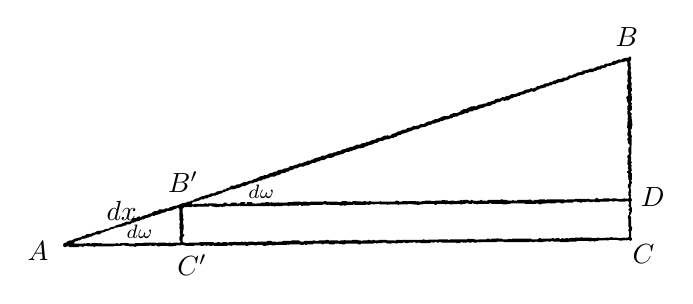
\begin{tikzpicture}[x=0.00703642cm,y=-0.00703642cm]
\fill[even odd rule] (1118,73) -- (1117,72) -- (1115,72) -- (1113,74) -- (1105,75) -- (1099,78) -- (1096,77) -- (1090,80) -- (1086,80) -- (1084,82) -- (1080,84) -- (1078,84) -- (1077,85) -- (1071,85) -- (1068,88) -- (1063,88) -- (1061,90) -- (1057,90) -- (1049,94) -- (1043,94) -- (1040,96) -- (1037,96) -- (1036,97) -- (1031,97) -- (1028,100) -- (1020,101) -- (1018,103) -- (1016,103) -- (1011,106) -- (1006,106) -- (1001,110) -- (995,110) -- (993,112) -- (985,113) -- (982,115) -- (979,115) -- (975,118) -- (971,118) -- (969,120) -- (961,121) -- (959,123) -- (956,123) -- (953,125) -- (949,125) -- (944,129) -- (942,129) -- (941,130) -- (937,129) -- (934,131) -- (927,132) -- (922,135) -- (914,137) -- (911,139) -- (908,139) -- (907,140) -- (902,140) -- (897,143) -- (893,143) -- (889,146) -- (886,145) -- (881,148) -- (876,148) -- (875,149) -- (873,149) -- (870,152) -- (867,152) -- (863,154) -- (860,154) -- (855,157) -- (851,157) -- (850,158) -- (843,159) -- (838,162) -- (836,162) -- (835,161) -- (833,162) -- (829,162) -- (826,164) -- (824,164) -- (820,167) -- (816,167) -- (812,169) -- (807,173) -- (805,173) -- (804,174) -- (797,174) -- (796,175) -- (792,176) -- (789,179) -- (778,180) -- (768,185) -- (764,185) -- (756,189) -- (752,189) -- (746,192) -- (744,194) -- (737,194) -- (735,196) -- (733,197) -- (730,197) -- (729,198) -- (725,197) -- (721,200) -- (714,201) -- (711,204) -- (706,204) -- (700,207) -- (697,207) -- (693,210) -- (686,212) -- (683,215) -- (679,215) -- (678,214) -- (676,215) -- (672,215) -- (665,219) -- (661,219) -- (660,220) -- (658,220) -- (656,222) -- (650,223) -- (644,226) -- (640,226) -- (638,228) -- (631,229) -- (629,231) -- (623,231) -- (615,235) -- (611,235) -- (608,237) -- (605,237) -- (602,239) -- (596,240) -- (592,243) -- (588,243) -- (584,245) -- (581,245) -- (578,247) -- (573,247) -- (565,251) -- (559,251) -- (557,253) -- (546,256) -- (543,258) -- (541,258) -- (539,260) -- (534,260) -- (531,262) -- (529,262) -- (523,265) -- (518,265) -- (515,267) -- (513,267) -- (506,270) -- (502,270) -- (499,273) -- (497,273) -- (496,274) -- (492,274) -- (488,276) -- (481,277) -- (477,280) -- (474,280) -- (470,282) -- (467,282) -- (460,286) -- (455,286) -- (453,288) -- (449,288) -- (440,293) -- (437,293) -- (433,296) -- (429,296) -- (428,297) -- (426,297) -- (424,299) -- (418,299) -- (410,303) -- (406,303) -- (403,305) -- (396,305) -- (392,309) -- (389,309) -- (387,311) -- (385,312) -- (382,312) -- (380,314) -- (369,316) -- (367,318) -- (365,318) -- (364,319) -- (359,319) -- (354,322) -- (350,322) -- (349,323) -- (341,325) -- (336,328) -- (333,328) -- (329,330) -- (327,332) -- (324,332) -- (321,334) -- (317,334) -- (314,336) -- (307,337) -- (298,341) -- (291,342) -- (290,343) -- (285,344) -- (283,346) -- (277,346) -- (275,348) -- (266,348) -- (264,350) -- (262,351) -- (258,351) -- (254,353) -- (252,355) -- (247,356) -- (244,358) -- (238,359) -- (234,361) -- (232,363) -- (230,361) -- (230,360) -- (229,361) -- (227,361) -- (224,364) -- (218,364) -- (216,365) -- (217,367) -- (213,370) -- (207,370) -- (206,371) -- (204,371) -- (202,373) -- (200,373) -- (196,375) -- (193,375) -- (192,376) -- (189,376) -- (185,379) -- (179,380) -- (174,383) -- (170,383) -- (164,386) -- (154,387) -- (149,390) -- (147,390) -- (143,392) -- (134,393) -- (132,395) -- (130,396) -- (127,396) -- (125,398) -- (113,401) -- (108,404) -- (104,404) -- (103,405) -- (101,405) -- (98,408) -- (94,409) -- (93,410) -- (92,414) -- (95,416) -- (97,416) -- (98,415) -- (103,415) -- (104,416) -- (120,416) -- (121,415) -- (126,415) -- (128,416) -- (131,414) -- (136,414) -- (137,415) -- (140,414) -- (141,415) -- (147,415) -- (149,416) -- (150,415) -- (153,415) -- (154,414) -- (156,415) -- (183,415) -- (184,414) -- (197,414) -- (198,413) -- (204,413) -- (205,414) -- (211,414) -- (212,415) -- (221,415) -- (222,416) -- (226,414) -- (244,414) -- (245,413) -- (247,414) -- (249,413) -- (251,413) -- (252,414) -- (257,414) -- (258,413) -- (260,413) -- (264,415) -- (267,415) -- (268,414) -- (282,414) -- (283,415) -- (286,415) -- (288,414) -- (290,415) -- (291,414) -- (295,414) -- (296,413) -- (305,413) -- (306,412) -- (309,412) -- (310,413) -- (313,413) -- (314,414) -- (328,414) -- (329,413) -- (340,413) -- (341,414) -- (345,414) -- (346,413) -- (350,413) -- (351,414) -- (353,413) -- (356,413) -- (357,414) -- (361,414) -- (362,413) -- (364,413) -- (365,414) -- (388,414) -- (389,413) -- (394,413) -- (396,414) -- (397,413) -- (400,413) -- (401,412) -- (403,412) -- (404,413) -- (422,413) -- (423,414) -- (425,414) -- (426,413) -- (430,413) -- (431,412) -- (436,412) -- (437,413) -- (442,413) -- (443,412) -- (451,412) -- (455,414) -- (458,414) -- (459,413) -- (463,413) -- (464,412) -- (468,412) -- (469,413) -- (475,413) -- (476,412) -- (496,412) -- (497,411) -- (499,412) -- (501,411) -- (520,411) -- (521,412) -- (526,412) -- (527,411) -- (529,411) -- (530,412) -- (532,412) -- (533,411) -- (543,411) -- (544,410) -- (559,410) -- (560,411) -- (562,411) -- (563,410) -- (572,410) -- (573,411) -- (582,411) -- (583,410) -- (591,410) -- (592,411) -- (594,410) -- (596,411) -- (601,411) -- (602,410) -- (624,410) -- (625,411) -- (629,411) -- (630,410) -- (652,410) -- (653,409) -- (657,409) -- (659,410) -- (660,409) -- (668,409) -- (669,408) -- (675,408) -- (677,410) -- (679,409) -- (681,410) -- (684,410) -- (685,409) -- (692,409) -- (694,410) -- (695,409) -- (705,409) -- (707,407) -- (711,409) -- (715,409) -- (716,408) -- (724,408) -- (725,407) -- (727,407) -- (730,409) -- (731,408) -- (737,408) -- (738,409) -- (754,409) -- (758,407) -- (760,408) -- (762,408) -- (763,407) -- (767,407) -- (768,408) -- (770,408) -- (771,407) -- (775,407) -- (776,408) -- (802,408) -- (803,409) -- (808,409) -- (811,407) -- (813,407) -- (814,408) -- (821,408) -- (822,407) -- (824,407) -- (825,408) -- (829,408) -- (830,407) -- (833,407) -- (834,408) -- (839,408) -- (840,407) -- (843,407) -- (845,408) -- (846,407) -- (875,407) -- (876,406) -- (887,406) -- (888,407) -- (934,407) -- (935,406) -- (937,406) -- (938,407) -- (944,407) -- (945,406) -- (948,406) -- (949,407) -- (959,407) -- (960,406) -- (965,406) -- (966,405) -- (968,406) -- (973,406) -- (974,405) -- (976,405) -- (977,406) -- (989,406) -- (990,407) -- (1005,407) -- (1006,406) -- (1019,406) -- (1020,405) -- (1041,405) -- (1042,406) -- (1050,405) -- (1051,406) -- (1053,406) -- (1054,405) -- (1058,405) -- (1059,404) -- (1069,404) -- (1070,403) -- (1072,404) -- (1077,404) -- (1078,403) -- (1093,403) -- (1094,404) -- (1098,404) -- (1099,405) -- (1101,404) -- (1106,404) -- (1107,403) -- (1109,404) -- (1113,403) -- (1117,405) -- (1119,403) -- (1119,400) -- (1118,399) -- (1118,387) -- (1119,386) -- (1119,383) -- (1120,382) -- (1118,378) -- (1118,368) -- (1117,367) -- (1118,362) -- (1116,360) -- (1116,358) -- (1118,356) -- (1118,354) -- (1119,353) -- (1119,345) -- (1118,344) -- (1118,333) -- (1119,332) -- (1119,330) -- (1117,326) -- (1117,324) -- (1118,323) -- (1117,321) -- (1117,319) -- (1118,318) -- (1117,316) -- (1118,314) -- (1117,312) -- (1117,306) -- (1118,305) -- (1118,302) -- (1119,301) -- (1119,298) -- (1118,297) -- (1118,295) -- (1119,294) -- (1119,283) -- (1118,282) -- (1118,279) -- (1119,278) -- (1118,271) -- (1119,269) -- (1118,268) -- (1118,265) -- (1119,263) -- (1117,260) -- (1118,258) -- (1118,253) -- (1117,252) -- (1117,250) -- (1118,249) -- (1119,215) -- (1118,214) -- (1118,207) -- (1117,206) -- (1117,204) -- (1119,202) -- (1119,198) -- (1120,197) -- (1120,193) -- (1119,191) -- (1120,189) -- (1119,188) -- (1119,185) -- (1118,184) -- (1119,182) -- (1118,180) -- (1119,175) -- (1116,172) -- (1116,171) -- (1119,168) -- (1119,161) -- (1118,160) -- (1119,158) -- (1119,156) -- (1118,155) -- (1118,152) -- (1119,151) -- (1119,144) -- (1118,143) -- (1119,141) -- (1118,139) -- (1118,135) -- (1119,134) -- (1119,129) -- (1118,128) -- (1119,120) -- (1118,119) -- (1118,116) -- (1117,115) -- (1119,110) -- (1118,109) -- (1118,100) -- (1117,99) -- (1117,94) -- (1118,92) -- (1117,91) -- (1117,84) -- (1116,83) -- (1116,81) -- (1118,77) -- cycle
(302,347) -- (302,351) -- (303,352) -- (302,354) -- (302,362) -- (303,363) -- (302,365) -- (302,367) -- (303,368) -- (303,373) -- (302,374) -- (303,379) -- (302,380) -- (302,382) -- (303,383) -- (303,392) -- (304,393) -- (303,397) -- (302,398) -- (302,403) -- (304,405) -- (304,407) -- (302,409) -- (300,408) -- (292,408) -- (291,409) -- (287,409) -- (286,408) -- (283,408) -- (282,409) -- (279,409) -- (278,408) -- (264,408) -- (263,409) -- (261,409) -- (260,408) -- (238,408) -- (237,409) -- (223,409) -- (222,410) -- (211,410) -- (210,409) -- (196,409) -- (195,410) -- (191,410) -- (190,409) -- (188,409) -- (187,410) -- (162,410) -- (161,409) -- (158,409) -- (157,410) -- (155,409) -- (144,409) -- (143,410) -- (141,410) -- (140,409) -- (135,409) -- (134,410) -- (132,410) -- (131,409) -- (129,410) -- (113,410) -- (112,409) -- (112,408) -- (114,406) -- (118,405) -- (119,404) -- (122,404) -- (127,401) -- (132,401) -- (135,399) -- (138,399) -- (140,397) -- (144,397) -- (146,395) -- (148,395) -- (151,393) -- (158,393) -- (162,390) -- (167,389) -- (170,387) -- (175,386) -- (178,384) -- (183,383) -- (186,381) -- (190,381) -- (191,380) -- (199,379) -- (200,378) -- (205,377) -- (207,375) -- (213,375) -- (217,372) -- (220,372) -- (223,370) -- (229,369) -- (235,366) -- (238,366) -- (241,364) -- (249,362) -- (253,359) -- (257,360) -- (259,358) -- (262,358) -- (263,357) -- (265,357) -- (272,354) -- (275,354) -- (280,351) -- (289,350) -- (294,347) -- (296,347) -- (298,345) -- (300,345) -- cycle
(1115,344) -- (1115,346) -- (1113,348) -- (1113,349) -- (1115,351) -- (1115,353) -- (1114,354) -- (1114,358) -- (1112,360) -- (1112,364) -- (1113,365) -- (1113,379) -- (1114,380) -- (1114,383) -- (1113,384) -- (1113,387) -- (1114,388) -- (1114,397) -- (1112,399) -- (1109,399) -- (1108,400) -- (1106,399) -- (1094,400) -- (1093,399) -- (1084,399) -- (1083,398) -- (1081,398) -- (1080,399) -- (1072,399) -- (1071,400) -- (1069,400) -- (1068,399) -- (1066,400) -- (1061,400) -- (1060,399) -- (1056,399) -- (1055,400) -- (1047,400) -- (1046,399) -- (1030,399) -- (1028,398) -- (1027,399) -- (1016,399) -- (1015,400) -- (1011,399) -- (1010,400) -- (1006,400) -- (1005,401) -- (1003,400) -- (1000,400) -- (999,401) -- (993,400) -- (991,402) -- (987,400) -- (983,400) -- (982,401) -- (979,401) -- (978,400) -- (975,400) -- (974,401) -- (955,401) -- (954,400) -- (952,400) -- (949,402) -- (938,402) -- (937,401) -- (903,401) -- (902,402) -- (896,401) -- (895,402) -- (886,402) -- (885,401) -- (878,401) -- (876,400) -- (875,401) -- (866,401) -- (865,402) -- (863,402) -- (862,401) -- (858,401) -- (857,402) -- (843,402) -- (842,403) -- (834,402) -- (833,401) -- (831,402) -- (829,401) -- (827,402) -- (825,401) -- (823,401) -- (822,402) -- (791,402) -- (790,403) -- (787,403) -- (786,402) -- (745,403) -- (744,402) -- (742,402) -- (741,403) -- (703,403) -- (702,404) -- (700,403) -- (694,403) -- (692,405) -- (690,404) -- (677,404) -- (676,403) -- (663,403) -- (662,404) -- (655,404) -- (654,403) -- (652,403) -- (651,404) -- (647,404) -- (646,403) -- (643,403) -- (642,404) -- (633,404) -- (632,405) -- (630,405) -- (629,404) -- (625,404) -- (624,403) -- (615,403) -- (614,404) -- (602,404) -- (600,403) -- (599,404) -- (593,404) -- (592,405) -- (589,405) -- (588,404) -- (575,404) -- (574,405) -- (571,403) -- (567,403) -- (566,404) -- (554,404) -- (553,405) -- (547,405) -- (546,404) -- (544,404) -- (543,405) -- (528,405) -- (527,406) -- (521,406) -- (518,404) -- (505,404) -- (504,405) -- (489,405) -- (488,406) -- (481,406) -- (480,407) -- (477,407) -- (476,406) -- (469,406) -- (468,405) -- (461,405) -- (460,406) -- (443,406) -- (442,407) -- (437,407) -- (436,406) -- (427,406) -- (426,407) -- (423,407) -- (422,406) -- (420,406) -- (419,407) -- (417,407) -- (416,406) -- (414,406) -- (413,407) -- (404,407) -- (402,406) -- (401,407) -- (392,407) -- (391,408) -- (388,408) -- (387,407) -- (381,407) -- (380,408) -- (375,408) -- (374,407) -- (371,407) -- (370,408) -- (367,408) -- (366,409) -- (365,409) -- (363,407) -- (339,407) -- (338,408) -- (320,408) -- (319,409) -- (314,409) -- (313,408) -- (310,408) -- (308,406) -- (308,399) -- (311,395) -- (311,394) -- (308,391) -- (309,389) -- (309,385) -- (310,384) -- (310,376) -- (309,375) -- (309,368) -- (310,366) -- (309,365) -- (309,357) -- (308,356) -- (308,347) -- (311,344) -- (316,344) -- (317,343) -- (319,344) -- (324,344) -- (325,343) -- (329,343) -- (330,344) -- (332,344) -- (333,343) -- (355,343) -- (358,341) -- (359,341) -- (361,343) -- (365,343) -- (366,344) -- (373,344) -- (374,343) -- (378,343) -- (380,344) -- (381,343) -- (384,343) -- (385,342) -- (392,342) -- (394,343) -- (395,342) -- (409,342) -- (410,341) -- (412,342) -- (465,342) -- (467,341) -- (468,342) -- (472,342) -- (474,343) -- (475,342) -- (488,342) -- (489,341) -- (497,341) -- (498,342) -- (500,342) -- (501,341) -- (518,341) -- (519,340) -- (521,340) -- (523,342) -- (524,342) -- (525,341) -- (537,341) -- (538,340) -- (560,340) -- (561,339) -- (567,339) -- (568,340) -- (571,340) -- (572,339) -- (574,340) -- (591,340) -- (592,341) -- (596,341) -- (597,340) -- (599,341) -- (603,341) -- (604,340) -- (615,340) -- (616,339) -- (618,339) -- (619,340) -- (638,340) -- (639,339) -- (645,340) -- (646,339) -- (649,339) -- (650,338) -- (652,339) -- (663,338) -- (664,339) -- (677,339) -- (678,340) -- (680,339) -- (696,339) -- (698,340) -- (699,339) -- (715,339) -- (716,338) -- (735,340) -- (736,339) -- (742,339) -- (743,338) -- (762,338) -- (764,340) -- (766,340) -- (768,338) -- (781,338) -- (782,339) -- (784,339) -- (785,338) -- (789,338) -- (790,339) -- (808,338) -- (809,339) -- (813,339) -- (814,338) -- (818,338) -- (819,337) -- (824,337) -- (825,338) -- (830,338) -- (831,337) -- (833,337) -- (834,338) -- (838,338) -- (839,339) -- (841,339) -- (842,338) -- (861,338) -- (862,337) -- (865,337) -- (866,338) -- (885,338) -- (886,339) -- (893,339) -- (894,338) -- (899,338) -- (900,337) -- (925,337) -- (926,338) -- (946,338) -- (947,337) -- (949,337) -- (952,339) -- (954,339) -- (955,338) -- (967,337) -- (968,336) -- (970,337) -- (981,337) -- (982,336) -- (990,336) -- (991,337) -- (996,337) -- (997,336) -- (1001,336) -- (1002,335) -- (1004,336) -- (1012,336) -- (1014,334) -- (1020,334) -- (1021,335) -- (1025,335) -- (1026,336) -- (1028,336) -- (1029,335) -- (1036,335) -- (1037,334) -- (1042,334) -- (1043,335) -- (1048,335) -- (1049,334) -- (1051,334) -- (1052,335) -- (1061,335) -- (1062,334) -- (1078,334) -- (1079,333) -- (1084,333) -- (1085,334) -- (1087,334) -- (1088,333) -- (1094,333) -- (1095,334) -- (1107,334) -- (1108,333) -- (1112,333) -- (1114,335) -- (1114,339) -- (1113,340) -- (1113,342) -- cycle
(1111,82) -- (1111,89) -- (1113,93) -- (1112,94) -- (1112,97) -- (1111,98) -- (1111,106) -- (1112,107) -- (1111,117) -- (1112,118) -- (1112,122) -- (1110,124) -- (1110,130) -- (1112,132) -- (1112,139) -- (1113,141) -- (1109,146) -- (1109,147) -- (1110,148) -- (1110,152) -- (1113,158) -- (1111,162) -- (1111,168) -- (1112,169) -- (1111,171) -- (1111,176) -- (1112,177) -- (1112,183) -- (1111,185) -- (1112,186) -- (1112,189) -- (1111,190) -- (1111,197) -- (1110,199) -- (1112,202) -- (1112,209) -- (1111,210) -- (1111,214) -- (1113,216) -- (1113,218) -- (1111,220) -- (1111,223) -- (1112,224) -- (1112,228) -- (1115,231) -- (1115,235) -- (1113,237) -- (1113,245) -- (1114,246) -- (1114,248) -- (1111,251) -- (1111,255) -- (1112,256) -- (1111,266) -- (1113,270) -- (1112,272) -- (1112,275) -- (1114,277) -- (1110,280) -- (1110,281) -- (1113,284) -- (1112,289) -- (1113,290) -- (1113,294) -- (1114,295) -- (1114,301) -- (1112,304) -- (1112,308) -- (1114,311) -- (1114,315) -- (1113,316) -- (1113,323) -- (1114,324) -- (1114,327) -- (1112,329) -- (1104,328) -- (1103,329) -- (1099,329) -- (1097,330) -- (1096,329) -- (1092,329) -- (1091,328) -- (1084,328) -- (1083,329) -- (1079,329) -- (1078,328) -- (1068,328) -- (1067,329) -- (1063,329) -- (1061,330) -- (1055,327) -- (1052,330) -- (1043,330) -- (1042,329) -- (1037,329) -- (1036,330) -- (1034,329) -- (1031,329) -- (1030,330) -- (1028,329) -- (1017,329) -- (1016,330) -- (1002,330) -- (1001,331) -- (998,331) -- (997,330) -- (966,330) -- (965,331) -- (963,331) -- (962,330) -- (952,330) -- (951,331) -- (943,331) -- (942,332) -- (939,332) -- (935,330) -- (933,331) -- (913,331) -- (912,332) -- (906,332) -- (905,331) -- (903,332) -- (895,332) -- (894,331) -- (887,331) -- (886,330) -- (883,330) -- (882,331) -- (860,331) -- (856,333) -- (854,332) -- (849,332) -- (848,331) -- (846,331) -- (845,332) -- (841,332) -- (840,333) -- (832,332) -- (831,331) -- (829,331) -- (827,333) -- (823,331) -- (815,331) -- (814,332) -- (810,331) -- (809,332) -- (805,332) -- (804,333) -- (799,333) -- (798,332) -- (792,332) -- (791,333) -- (788,333) -- (787,332) -- (777,331) -- (776,332) -- (765,332) -- (764,333) -- (757,333) -- (756,332) -- (746,332) -- (745,333) -- (741,333) -- (740,334) -- (734,334) -- (733,333) -- (731,334) -- (729,333) -- (716,333) -- (715,334) -- (713,333) -- (705,333) -- (704,334) -- (699,334) -- (698,333) -- (694,332) -- (691,334) -- (667,334) -- (665,333) -- (664,334) -- (655,334) -- (654,335) -- (652,334) -- (648,334) -- (647,333) -- (645,333) -- (644,334) -- (639,334) -- (638,333) -- (635,333) -- (634,334) -- (616,333) -- (613,335) -- (611,334) -- (605,334) -- (604,333) -- (596,333) -- (594,335) -- (589,335) -- (588,334) -- (568,334) -- (567,333) -- (564,333) -- (563,334) -- (539,334) -- (538,335) -- (533,335) -- (532,334) -- (526,334) -- (525,335) -- (522,335) -- (521,334) -- (508,334) -- (507,335) -- (498,335) -- (497,336) -- (482,336) -- (481,335) -- (479,336) -- (470,336) -- (469,335) -- (467,336) -- (464,336) -- (463,335) -- (458,335) -- (457,336) -- (450,336) -- (449,337) -- (442,337) -- (441,338) -- (439,338) -- (438,337) -- (436,337) -- (435,338) -- (433,336) -- (434,335) -- (424,335) -- (425,336) -- (423,338) -- (421,338) -- (420,337) -- (420,336) -- (422,335) -- (413,335) -- (412,337) -- (409,337) -- (408,338) -- (407,338) -- (405,336) -- (396,336) -- (394,338) -- (389,338) -- (387,336) -- (383,336) -- (381,338) -- (369,338) -- (368,337) -- (366,338) -- (364,337) -- (355,337) -- (354,338) -- (352,338) -- (351,337) -- (348,337) -- (347,338) -- (330,338) -- (329,339) -- (326,339) -- (324,337) -- (328,334) -- (332,334) -- (333,333) -- (338,332) -- (341,330) -- (346,330) -- (348,328) -- (353,328) -- (355,326) -- (357,326) -- (364,323) -- (368,323) -- (369,322) -- (371,322) -- (374,320) -- (379,319) -- (381,317) -- (384,317) -- (386,315) -- (388,315) -- (394,312) -- (398,312) -- (399,311) -- (401,312) -- (402,311) -- (413,308) -- (415,306) -- (420,306) -- (430,301) -- (434,301) -- (438,299) -- (441,299) -- (446,296) -- (450,296) -- (453,294) -- (456,294) -- (459,292) -- (462,292) -- (467,289) -- (474,289) -- (477,287) -- (484,285) -- (486,283) -- (488,283) -- (489,282) -- (493,282) -- (496,280) -- (499,280) -- (501,278) -- (503,277) -- (506,277) -- (510,274) -- (514,274) -- (520,271) -- (526,271) -- (529,269) -- (535,268) -- (543,264) -- (547,264) -- (550,262) -- (555,261) -- (558,259) -- (563,259) -- (570,255) -- (577,255) -- (578,254) -- (580,254) -- (584,251) -- (587,251) -- (588,250) -- (591,250) -- (592,249) -- (597,248) -- (604,244) -- (609,244) -- (610,243) -- (613,243) -- (616,241) -- (618,241) -- (625,238) -- (630,238) -- (631,237) -- (634,237) -- (639,234) -- (642,234) -- (644,232) -- (650,231) -- (656,228) -- (659,228) -- (663,225) -- (670,224) -- (673,222) -- (681,221) -- (685,219) -- (689,219) -- (691,217) -- (694,217) -- (696,215) -- (698,214) -- (701,214) -- (705,211) -- (708,211) -- (709,210) -- (714,209) -- (717,207) -- (720,207) -- (725,204) -- (734,203) -- (738,200) -- (746,199) -- (752,196) -- (757,195) -- (759,193) -- (763,193) -- (767,191) -- (770,191) -- (775,188) -- (778,188) -- (782,186) -- (789,185) -- (790,184) -- (795,183) -- (797,181) -- (805,180) -- (807,178) -- (809,178) -- (810,177) -- (812,177) -- (819,174) -- (823,174) -- (826,171) -- (831,171) -- (834,169) -- (838,169) -- (844,166) -- (852,164) -- (855,162) -- (863,161) -- (868,158) -- (871,158) -- (875,155) -- (881,154) -- (885,151) -- (887,151) -- (888,152) -- (890,152) -- (891,151) -- (896,151) -- (902,147) -- (904,147) -- (907,145) -- (910,145) -- (914,143) -- (917,143) -- (919,141) -- (925,140) -- (930,137) -- (933,137) -- (937,135) -- (940,135) -- (942,136) -- (946,134) -- (948,132) -- (951,132) -- (953,130) -- (959,129) -- (960,128) -- (963,128) -- (965,126) -- (968,126) -- (971,124) -- (974,124) -- (976,122) -- (981,122) -- (983,120) -- (985,120) -- (986,119) -- (994,118) -- (999,115) -- (1002,115) -- (1006,113) -- (1008,111) -- (1014,110) -- (1015,109) -- (1018,109) -- (1020,107) -- (1024,106) -- (1025,105) -- (1030,105) -- (1034,103) -- (1036,101) -- (1039,102) -- (1042,100) -- (1049,100) -- (1051,98) -- (1054,98) -- (1057,96) -- (1063,95) -- (1065,93) -- (1072,92) -- (1075,89) -- (1081,89) -- (1083,87) -- (1088,87) -- (1091,85) -- (1093,85) -- (1095,83) -- (1098,83) -- (1099,82) -- (1104,82) -- (1109,80) -- cycle;
\node[inner sep=0pt,font=\fontsize{10}{12}\selectfont] at (1110,37) {$B$};
\node[inner sep=0pt,font=\fontsize{10}{12}\selectfont] at (309,298) {$B'$};
\node[inner sep=0pt,font=\fontsize{10}{12}\selectfont] at (198,351) {$dx$};
\node[inner sep=0pt,font=\fontsize{7}{9}\selectfont] at (230,388) {$d\omega$};
\node[inner sep=0pt,font=\fontsize{7}{9}\selectfont] at (450,317) {$d\omega$};
\node[inner sep=0pt,font=\fontsize{10}{12}\selectfont] at (47,423) {$A$};
\node[inner sep=0pt,font=\fontsize{10}{12}\selectfont] at (325,449) {$C'$};
\node[inner sep=0pt,font=\fontsize{10}{12}\selectfont] at (1157,326) {$D$};
\node[inner sep=0pt,font=\fontsize{10}{12}\selectfont] at (1140,429) {$C$};
\end{tikzpicture}


Fig. 12.
\end{minipage}\end{center}

Trägt man auf $AB$ die Strecke $AB' = dx$ ab und fällt von $B'$ auf $AC$ das Loth
$C'$, so ist wieder nach (A'):
\[
BD = f(x) \,.\, d\omega, \qquad C'B' = f(dx) \,.\, d\omega.
\]
Errichtet man endlich auf $B'C'$ in $B'$ das Loth $B'D$, das $BC$ in $D$ trifft,
so ist nach B):
\[
CD = g(C'C) \,.\, C'B',
\]
also, da $C'C$ sich von $B'B$ nur unendlich wenig unterscheidet:
\[
\tag*{11)} CD = g(x) \,.\, f(dx) \,.\, d\omega,
\]

